\documentclass[twocolumn,preprintnumbers,amsmath,amssymb,superscriptaddress]{revtex4}
%\usepackage[pdftex]{graphicx}

\usepackage{amsmath,amsfonts,amssymb}
\usepackage[english]{babel}
\usepackage[latin1]{inputenc}
\usepackage[T1]{fontenc}
\usepackage{color}
\usepackage{float}
\usepackage{verbatim}
\usepackage{graphicx}
\usepackage{bm}
\usepackage{mathtools}
\usepackage{stmaryrd}
\usepackage{anyfontsize}


\graphicspath{{../Enigma/figures/}}
\newcommand{\rr}[1]{{\rm #1}}

%\usepackage{epstopdf}
%\usepackage{array}
%\usepackage{tabularx}
%\usepackage{multirow}
\usepackage{color}
%\usepackage{multibox}
%\usepackage{rotating}
%\usepackage{lineno}
%\usepackage[left]{lineno}
%\usepackage[comma,sort&compress]{natbib}
%\usepackage{authblk}
%\usepackage{multicol}

%\bibliographystyle{ieeetr}


%\linenumbers
%\setlength\linenumbersep{3pt}

\begin{document}



\author{Justin D. Yeakel} \affiliation{School of Natural Sciences, University
  of California, Merced, Merced, CA 95340, USA}

\author{Mathias Pires} \affiliation{}

\author{James O'Donnell} \affiliation{}

\author{Marcus de Aguiar} \affiliation{}

\author{Paulo Guimar\~aes Jr} \affiliation{}

\author{Dominique Gravel} \affiliation{}

\author{Thilo Gross} \affiliation{}

%\title{Simple rules yield complex communities: deconstructed species interactions and the assembly of communities}
%\title{Community assembly and dynamics by the deconstruction of species interactions}
\title{Quantization of ecological interactions yields insights into food web assembly and dynamics}
%\author{Justin D. Yeakel${}^{1,2,*}$, Christopher P. Kempes${}^{2}$, \& Sidney Redner${}^{2,3}$ \\ \\
%${}^1$School of Natural Science, University of California Merced, Merced, CA \\
%${}^2$The Santa Fe Institute, Santa Fe, NM \\
%${}^3$Department of Physics, Boston University, Boston MA \\
%${}^*$To whom correspondence should be addressed: jdyeakel@gmail.com
%}


\begin{abstract}
  The dynamics of community assembly has a rich history in ecological theory. Recently, there has been much interest in assessing how changes in diversity within assembling communities impact the structure of interactions and vice versa. 
  Here we examine a novel theoretical framework that seeks to generate communities by distilling many types of ecological interactions into a small number of unique pairwise directed links between species, including, but not limited to, `assimilate' interactions (e.g. resource dependencies) and 'need' interactions (e.g. reproductive or habitat dependencies). 
  Different pairwise combinations of directed link types between species give rise to the larger diversity of species interactions observed in nature, such as consumer-resource, and both service-resource and service-service mutualisms. 
  Moreover, our framework permits the explicit inclusion of interactions that create or modify abiotic elements, which other species may depend on for survival, such as nutrients or habitat. 
  Inclusion of both biotic and abiotic agents permits more complex and indirect interdependencies between species, effectively incorporating the concept of ecosystem engineering into interaction networks, where the environment can be altered by a species or groups of species, thereby facilitating or inhibiting the colonization of others.
  Our framework makes specific predictions that are borne out by observations in the field. First, we find that communities initially exhibit higher connectance (link density), which is quickly eroded to empirically observed values as competition for resources increases exclusion. 
  Niche overlap among species follows similar trends: there is initially a greater degree of overlap between species, and as the system settles to a steady state, this overlap becomes minimized, mirroring observations of assembly in natural grasslands. 
  Importantly, we find that an increase in the number of engineering species, by creating a greater number of direct and indirect interdependencies, constrains the assembly of communities initially, yet promotes assembly as the system matures. 
  This leads to communities that exhibit greater diversity, however the increased species richness facilitated by engineers comes at a cost: as the number of engineers grows early in the assembly process, extinction cascades become larger. 
  Our framework shows that despite the complexity of real communities, some of the most remarkable processes and patterns such as competitive exclusion, resource complementarity and extinction cascades, can be generated by simple interaction rules. 
  Moreover our findings indicate that ecosystem engineering might be an important component that is overlooked in ecological network theory.
\end{abstract}

\maketitle

\section*{Introduction}

%Food webs and mutualistic nets are components of larger communities


%Each species interacts in a specific way, without regard to the reciprocal effect on its interacter


%Both biotic and abiotic interactions alter the environment.
%Enviromental alterations of this engineering have longer timescales than the engineers themselves



%Species interactions have statistical properties, but these are outcomes of an assembly process.
%Simple assembly rules can predict certain structural attributes
%Multiple interaction types and engineering must be considered, given their obvious ubiquity


%Here we...



What do we gain by focusing on community dynamics rather than population dynamics?
By assuming that all species present in a community have achieved a steady state, we focus instead on those factors that

\section*{Model Description}

%The scale of the model
% \textbf{The ANIMe Model} We examine assembly and dynamics of communities where we consider the interaction constraints determining colonization and extinction of species.
% The underlying dynamic that determines whether a species can colonize the community lies in the extent to which its various interactions with other species are satisfied.
% As such, the ANIMe model tracks the presence/absence of species over time, but does not incorporate changes in abundance.
% We assume that the abundance of all species in a given community are $>0$ and infer persistence based on the combination of interactions between species.
\textbf{The ENIgMa Model} We seek to understand the compound nature of species interactions by describing them by a limited set of directional interactions that are combined to represent an ecological relationship.
We aim to examine how these interdependencies between species in communities either aid or inhibit both assembly and extinction over long timescales, and specifically how ecosystem engineers contribute to these dynamics.
We approach these questions by considering multiple types of directional interactions between species, which, when paired represent specific ecological relationships including trophic interactions, service-resource and service-service mutualisms, and commensalisms.
We also introduce two types of nodes in our depiction of ecological networks: species and objects.
Objects are made by species (here and henceforth refereed to as engineers) and represent a modification to the available niche-space for other species in the community, including but not limited to: an introduced compound, metabolite, or alteration to the habitat/environment.



\begin{figure}
\centering
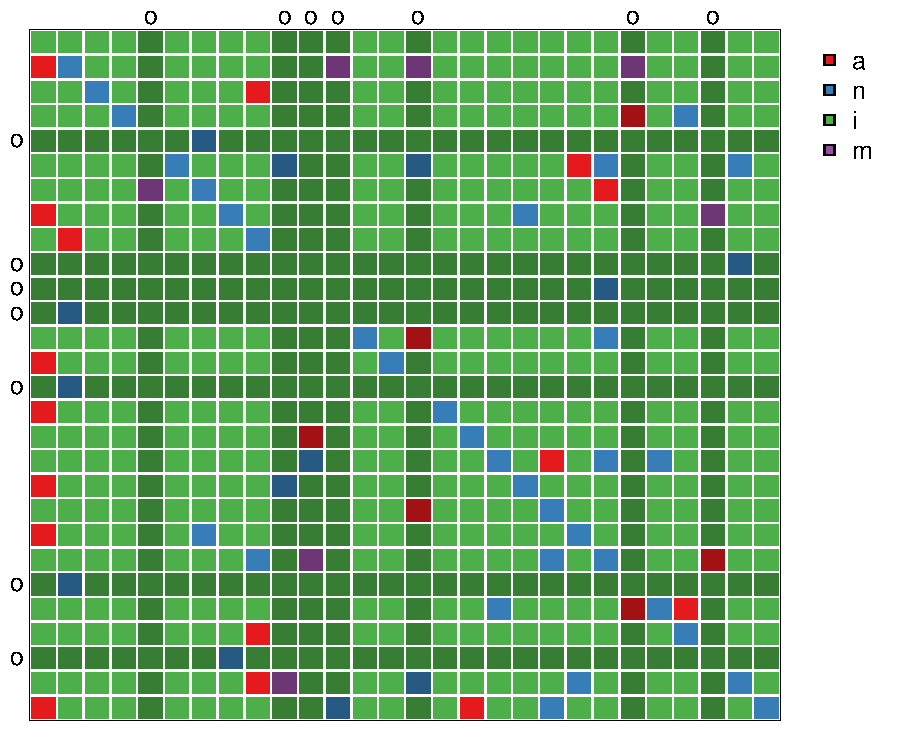
\includegraphics[width=0.45\textwidth]{matrix.pdf}
\caption{
An example of the source pool interaction matrix where $\mathcal{S} = 50$. Species and objects are aligned across the rows and columns; objects are shaded and labeled by `o' to distinguish them from species. The interaction recorded in row $i$ and column $j$ describes the directed interaction from species/object $i$ to species/object $j$. The first row/column represents the basal resource; species that assimilate the primary resource are capable of primary production. Species interact with other species and/or objects; objects only interact with their engineers by `needing' them; objects do not interact with other objects.
}
\label{fig:matrix}
\end{figure} 

%Interaction types

The ENIgMa model consists of four directed interactions:
$\rr{e}$: eat, which specifies a dependency involving the exchange of biomass,
$\rr{n}$: need, which specifies a dependency that does not involve biomass flow (e.g. a reproductive service),
$\rr{i}$: ignore, the null interaction, and
$\rr{m}$: make, which connects a species to an object that it engineers. 
`Objects' are interactive components that can be made by $\geq 1$ species, and eaten, needed, or ignored by the others.
The four directed interaction types describe specific dependencies that one species/object has on another, however it is the coupling of two opposing directed interactions that describe familiar ecological relationships (Table 1).

The $\rr{e} \leftrightarrow \rr{i}$ interaction describes a typical predator-prey relationship, where species 1 eats species 2, whereas aside from serving as a resource, species 2 does not interact with (ignores) species 1.
Of course, a prey's abundance does not \emph{ignore} the effects of predation, however our framework operates at the scale of presence/absence rather than abundance, and we assume that if both species co-occur, they have positive population densities, such that the prey's state (presence/absence) ignores the predator.
A second type of trophic interaction is described by $\rr{e} \leftrightarrow \rr{e}$, where consumption is symmetric, which could be do to changing roles over the lifetime of an individual.
The $\rr{e} \leftrightarrow \rr{n}$ and $\rr{n} \leftrightarrow \rr{n}$ interactions describe service-resource and service-service mutualisms, respectively.
In the case of the former, one species interacts by way of a trophic interaction, whereas the other is provided a non-trophic need, such is the case in a plant-pollinator relationship.
Unique to models of ecological networks, the $\rr{m} \leftrightarrow \rr{n}$ interaction describes ecosystem engineering, where a species makes an object, whereas the presence of the object `needs' the presence of the species that makes it.
Objects can be utilized by other species in the community, providing an indirect dependency that could be facilitated by multiple species (many engineers make the same object) and/or used by multiple species (many species eat or need the same object).
As we will describe below, engineers modify the niche space available to the community on timescales that last longer than the species themselves.

We explore the assembly of a novel community that emerges from a species source pool, which is represented by a source pool interaction matrix where all eat, need, ignore, make interactions are established between all species and objects.
As such, a set of interactions for a particular species defines how it interacts with any other \emph{a priori}, thereby establishing its potential interaction niche space.
The source pool is used to seed a novel community, which arises as the result of colonization and extinction rules, the details of which we describe below.



\textbf{Building the source pool} The source pool interaction matrix $\bm P$ is generated by first setting the number of species in the pool $\mathcal{S}_{\bm P}$ and determining the number of objects $\mathcal{O}_{\bm P}$ that are made by ecosystem engineers.
The resulting matrix is $\mathcal{N}_{\bm P}\times\mathcal{N}_{\bm P}$ where $\mathcal{N}_{\bm P}=\mathcal{S}_{\bm P}+\mathcal{O}_{\bm P}$, and is subdivided into four quadrants, only two of which play a role here: species-species interactions and species-object interactions (see Fig. \ref{fig:matrix}).
In each quadrant, the expected frequency of eat interactions ${\rm E}\{p_\rr{e}\}$ and the expected frequency of need interactions ${\rm E}\{p_\rr{n}\}$ are free parameters, as is the expected number of objects made per species ${\rm E}\{\mathcal{O}_i\}=\eta$.
Here and throughout, we simplify this parameter space by assuming that the frequency of eat and need interactions for species-species (SS) interactions and species-object (SO) interactions scale as $\phi$, such that ${\rm E_{SS}}\{p_\rr{e}\} = \phi{\rm E_{SO}}\{p_\rr{e}\}$ and ${\rm E_{SS}}\{p_\rr{n}\} = \phi{\rm E_{SO}}\{p_\rr{n}\}$.
% is given by the parameter ${\rm E}\{\mathcal{O}_i\}=\eta$, which determines how many objects will be present in the source pool.
% The source pool interaction matrix $\bm P$ is generated by first setting the number of species $\mathcal{S}$ and the expected number of objects that are engineered per species ${\rm E}\{\mathcal{O}_i\}=\eta$.
For each species, a set number of objects is drawn from ${\rm Poiss}(\eta)$, such that the expected proportion of species that are engineers (species that make objects) is $1-{e}^{-\eta}$. 
If a particular object is randomly and independently drawn for a given engineer from a complete list of all possible objects, such that multiple species -- with some probability -- can make the same object, the expected number of objects is
\begin{equation}
{\rm E}\{\mathcal{O}_{\bm P}\} = \mathcal{S}_{\bm P}\eta\left(1 - \frac{1}{{e}}\right),
\end{equation}
where $e$ is Euler's number.
% This allows multiple species to make the same object.
% If each species makes unique objects, the number of expected objects is $\mathcal{O} = \mathcal{S}\eta$, however because multiple species can make the same object, the realized number of objects will be lower.
% % To determine whether objects are uniquely made or made by multiple engineers, we assign objects by randomly drawing independently object IDs from $[1:\mathcal{O}_{\rm max}]$ without replacement for each engineer; unassigned objects are discarded.
% Each engineer is randomly assigned an object, which permits a single object to be made by multiple engineers, such that
% \begin{equation}
% {\rm E}\{\mathcal{O}\} = \mathcal{S}\eta\left(1 - \frac{1}{{\rm e}}\right).
% \end{equation}
% where $\rm e$ is Euler's number.
The frequency of $m \leftrightarrow n$ interactions is then calculated as
\begin{equation}
{\rm E}\{p_\rr{m}\} = \frac{\eta}{\mathcal{S}_{\bm P}\left(1 + \eta - \frac{\eta}{e}\right)^2}.
\end{equation}
Finally the frequency of the ignore interaction is calculated as $\rr{E_{SS}}\{p_\rr{i}\} = 1 - \rr{E_{SS}}\{p_\rr{e}\} + \rr{E_{SS}}\{p_\rr{n}\}$ and  $\rr{E_{SO}}\{p_\rr{i}\} = 1 - \rr{E_{SO}}\{p_\rr{e}\} + \rr{E_{SO}}\{p_\rr{n}\}+ \rr{E_{SO}}\{p_\rr{m}\}$ for species-species and species-object interactions, respectively.
Pairwise interaction probabilities between both species and objects are then calculated as shown in Table \ref{table:param}.
These pairwise interactions are assigned randomly between species and objects independently in both quadrant, such that the source pool matrix has no imbued structure apart from the number of species, the number of objects, and the frequency of each directional interaction type.
Each source pool is provided a \emph{basal resource} (the first row/column).
A species with a single trophic interaction to this resource is identified as a primary producer (Fig. \ref{fig:matrix}), however the basal resource does not have eat, need, or make interactions itself.


\textbf{Colonization and Extinction} Assembly of a species community is the result of both local colonization and extinction of species that are drawn from the source pool.
The realized interactions within the assembled community $\bm A$ are thus a subset of the potential interactions observed if every species were present (as recorded in the source pool $\bm P$). 
% though not all species can necessarily coexist in an assembled community at a given time.
We determine the ability of a species to colonize a community as a function of two conditions:
1) the colonizing species must eat \emph{at least one} species/object in the community, and
2) the colonizing species must satisfy all of its need interactions; if these conditions are both satisfied, colonization is possible.
At each time-step, one potential colonizer that fulfills these conditions is selected at random and added to the community, as well as the objects that it makes if it is an engineer.
Thus, in the first time-step, only species that consume the primary resource (row 1; figure \ref{fig:matrix}) and do not have any `need' interactions can initiate the assembly process.

% \begin{figure}
% \centering
% \includegraphics[width=0.4\textwidth]{predpreymotif.pdf}
% \caption{
% Non-specialist predators ($q=2$) consume a shared resource $i$, while each has alternative resources to fall-back on. Assuming Lotka-Volterra dynamics and equivalent attack rates of the predators $\beta$, the non-dimensional steady state density for the shared resource is $r_i^* = R_i^*/\kappa_i=1 - q\epsilon_i$ where $\epsilon_i=\beta P^*/\alpha_i$. We use this relationship between resource density and the number of predators $q$ to calculate extinction probabilities as a function of the number of predators $\omega_i(q)$
% }
% \label{fig:lv}
% \end{figure} 

%Extinction
Extinction occurs directly via competitive exclusion, or indirectly via the subsequent loss of a consumer's single resource or any of the species/objects it needs.
Extinction due to competitive exclusion is determined by violation of a single condition: a species must be the strongest competitor for at least one of its food resources.
% This requires a definition of a species' competitive strength $\sigma_i$.
In a given community, each species $i$ has a competition strength $\sigma_i$ that is compared to that for every species $j$ that shares its resources.
If $\sigma_i$ is not the highest $\sigma$ for at least one its resources, then species $i$ is competitively excluded from the community along with all unique objects that it makes.
The competition strength for species $i$, $\sigma_i$, increases as the sum of its potential need interactions, and decreases as both the sum of its potential eat interactions and the sum of its realized predators, such that 
\begin{equation}
  \sigma_i = \pi \sum_{j=1}^{\mathcal{N}_{\bm P}} \rr{n}_{{\bm P}(i,j)} - \sqrt{2}\sum_{j=1}^{\mathcal{N}_{\bm P}} \rr{e}_{{\bm P}(i,j)} - \sum_{i=1}^{\mathcal{N}_{\bm A}} \rr{e}_{{\bm A}(i,j)},
\end{equation}
where the summations describe the number of need interactions, eat interactions, and predators, respectively, and $\mathcal{N}_{\bm A} = \mathcal{S}_{\bm A} + \mathcal{O}_{\bm A}$ is the size of the assembled community $\bm A$ as the sum of the number of species and objects. 
The coefficients serve only to prevent the substitution of different interaction types.
Why do we assume that mutualisms increase a species' comepetitive strength?
Although mutualisms serve to tie the existence of one species to another, which increases its risk exposure, we assume that this dependency evolved as the consequence of a fitness advantage inherent in the interaction, providing a competitive edge.
% For example, a plant dispersing pollen through a pollinator compared to a plant dispersing pollen by air would be expected -- all else equal -- to have a competitive advantage.
Conversely, we assume that specialists (species with fewer trophic interactions) are competitively superior to generalists (ref), and that as a species spends more energy avoiding predation, it spends less energy competing.
Importantly, we emphasize that the role of mutualisms and trophic interactions in determining a species' competition strength is with respect to its \emph{potential} interaction niche, and thus calculated from the source pool matrix $\bm P$, whereas its vulnerability to predation is determined by a species' predators within the assembled community $\bm A$.
Therefore, the first two factors of $\sigma_i$ (the influence of its need and eat interactions) are independent of the community, whereas its vulnerability changes with community structure.
We note that due to the threshold conditions for colonization, $\sum_{j=1}^{\mathcal{N}_{\bm P}} \rr{n}_{{\bm P}(i,j)} = \sum_{j=1}^{\mathcal{S}_{\bm A}} \rr{n}_{{\bm A}(i,j)}$.

We integrate these colonization and extinction rules to simulate community assembly over time using a Gillespie algorithm.
At each time-step a single event is chosen at random to iterate the simulation forward, where possible event types include: 1) species colonization, 2) species extinction, and 3) object extinction.
The likelihood of drawing each event increases with the number of potential colonizers ($n_c$) or the number of species ($n_e$) and objects ($n_o$) that meet the conditions required for extinction.
The change in time $\rr{dt}$ at each step in the simulation is therefore dynamic, where $\rr{dt} = 1/\sum_i k_i(t)$ where $k_i(t)$ is the number of possible events of type $i$ at time $t$.
This algorithm allows, with some probability, that both species and objects to remain in the system after they are selected for extinction, however this probability declines as the rate of colonization (number of potential colonization events, $n_c$) decreases and the rate of extinction (number of potential extinction events, $n_e + n_o$) increases.
To incorporate the idea that the timescale of objects in a system should be longer than the timescale of the engineers that made them, we bias the algorithm to select a colonization or species extinction event with weight $\tau$.
If $\pi_e = n_e/n$ and $\pi_o = n_o/n$, species extinction occurs with probability $\tau \pi_e/(\tau \pi_e + (1-\tau)n_o)$ vs. an object extinction event that occurs with probability $(1-\tau) n_o/(\tau n_e + (1-\tau)n_o)$: as $\tau$ increases, the likelihood that an object is eliminated from the system declines.
% As we will discuss, this is an important attribute of ecosystem engineering that this particular framework allows us to explore.


\section*{Results}
%Food webs

\textbf{Diverse interactions without engineers} Community assembly in the absence of engineers ($\eta=0$) reveals the emergence of food web and mutualistic web properties consistent with observations of steady state and assembling empirical systems.
We set $S_{\bm P}=200$, $p_\rr{e}=0.01$, $p_\rr{n}=0.002$, and $t_\rr{max}=4000$.
Because only primary producers that do not have outgoing need interactions can colonize initially, a diverse base of these autotrophs typically constitutes the early assembly process.
In order for communities to have $>1$ pure autotroph, we do not consider competitive exclusion of the basal resource, such that all non-mutualistic pure autotrophs have the potential to coexist.
Following the establishment of a suite of autotrophs, both mixotrophs and low trophic-level heterotrophs assemble into the community, and competitive exclusion begins to increase the extinction rate.
It is with the establishment of higher-trophic level consumers that the rate of extinction begins to approximate the rate of colonization, such that community diversity begins fluctuating around a steady state.
This community steady state increases as the number of mutualisms established in the source pool decreases (lower $\rr{E}\{p_\rr{n}\}$) because mutualisms introduce dependencies that prevent colonization.

% 1) connectance
As the community assembles, we find that the connectance of trophic interactions ($C=L/S^2)$ where in our case $L=\sum_{i,j} \rr{e}_{{\bm A}(i,j)}$ and $S = \mathcal{S}_{\bm A}$) follows a decay-like trajectory to values similar to -- but on average 9\% greater than -- the connectance of the source pool $\bm{P}$.
% The species richness of the community increases to $S_{\bm A}=130$.
Decaying connectance has been documented in the assembly of mangrove communities (Piechnik), however this decay is a statistical inevitability, as a growing food web early in the assembly process undergoes both increasing species richness (to a mean steady state value of $S^*_{\bm A}=130$ species) and - through the establishment of different trophic levels and compartments - a decline in link density relative to the small, densely connected network at the beginning of assembly.
That the connectance of assembled communities is greater than the source pool is due to the fact that only species connected by trophic interactions can enter the community to begin with, increasing expected link density compared to the overall pool.


% 2) degree distributions
% a) realized vs. potential mean trophic degrees
% b) initially consumers are feeding as specialists
% c) generalist interactions become more prevalent as the system grows
% d) The mature food web has a skewed degree distribution with many specialists and a longer tail of generalist interactors

% Because only primary producers without outgoing mutualistic interactions can enter the community at the beginning of the assembly process, trophic specialists (as measured by the number of trophic interactions) are initially dominant.
% Because species are drawn from a source pool they possess both realized trophic interactions as well \emph{potential} trophic interactions, which defines their potential dietary flexibility as species colonize the system.
% Early in assembly, the mean number of realized trophic interactions among species is unity due to autotrophic bias, however the trophic potential of these early colonizers is highly variable (Fig. \ref{fig:spec}a).
% Thus although species assembling into the nascent community are functionally specialists, their potential trophic breadth is more broadly distributed than those species that colonize later in assembly.

% As the community assembles, we observe that the mean number of realized trophic interactions of species increases as a larger proportion of each species' trophic potential is realized with community size.
% However it is desirable to scale the definition of a specialist/generalist consumer to the link density of the food web.

% Prior observations have suggested that generalists dominate the initial assembly process, and specialists colonize later, causing food web connectance to decline. 
The trophic breadth of species is thought to play an important role in community assembly, and while many measure exist, trophic generality can be defined as $G_i = \sum_j \rr{e}_{{\bm A}(i,j)}(L/S)^{-1}$, such that the number of trophic interactions for a consumer is scaled by the average number of trophic interactions per species in the community $L/S$.
A species is classified as a generalist if the number of its trophic interactions is greater than the average number of links per species, or $G_i > 1$, and a specialist if $G_i < 1$, where a community can be described by its proportion of specialists $\rho_\rr{s}(G)$.
Thus, $G_i$ is scaled to the average number of trophic links among species, such that the trophic breadth of species in communities of difference size and/or connectance can be directly compared.
Piechnik et al. scales trophic breadth to a standard steady state value of $L^*/S^* = 0.2$ averaged across 102 food webs, and we refer to this measure of generality as $G_i^*$.
However, if we assume that $L/S$ is measured with respect to current community composition, $S = \mathcal{S}_{\bm A}$ and $L=\sum_{i,j} \rr{e}_{{\bm A}(i,j)}$ [MORE HERE].
% Piechnik et al. (2008) report the proportion of specialists in assembling communities over time, but where a species' trophic interactions are scaled by the steady state $L/S = L^*/S^*$ averaged across 102 food webs.
% Because communities early in the assembly process are by definition small, the value of $G_i$ is particularly sensitive to the scalar $L/S$: in the case of an assembling system, we could either employ a measure of $L/S$ representative of the current state of the system, or the steady state of the system.
% To compare our measure of generality with that employed by Piechnik et al. (2008), we must additionally consider which species are included in the measure of $S$ and $L$, as five autotrophic taxa were included in their empirical data, whereas our asssembly model may permit greater autotrophic diversity.
To address differences in scaling generalism against the average number of trophic links per species, we employ three different measures of $L/S$ to calculate $G_i$ and determine changes in the proportion of specialists in food webs over the course of assembly:
1) $G_i^{\rr{all}}$, where $L$ accounts for all links in the food web and $S$ accounts for all species relative to each time interval in the assembly process (circles; Fig. \ref{fig:spec}b);
2) $G_i^{\rr{hetero}}$, where we consider only the links and species richness of heterotrophs, excluding autotrophs (points; Fig. \ref{fig:spec}b);
3) $G_i^*$, where $L$ and $S$ are measured with respect to the communities at steady state (closest to Piechnik et al., 2008; diamonds; Fig. \ref{fig:spec}b).


Whether trophic breadth is scaled to the current state of $L/S$ or the steady state value of $L^*/S^*$ has a large effect on the estimated proportion of generalists in the community, particularly when the size of the system is small.
We observe that for $G_i^{\rr{all}}$, the system is initially assembled by specialist species, but where the proportion of specialists relative to generalists declines to ca. 60\% by the time the community reaches steady state.
If only the trophic links between heterotrophs are considered as in $G_i^{\rr{hetero}}$, specialists still dominate early in assembly, but there is a greater range, such that some systems can be described by a mixed proportion of specialists and generalists.
If generalism is measured with respect to the steady state $L^*/S^*$ as in $G_i^*$, we observe that generalists dominate early in assembly.
% In all cases, we observe that the colonization/extinction dynamic employed by the ENIgMa model results in a similar proportion of generalists and specialists as observed in Piechnik et al. (2008).

%Trophic Levels & degree dists
The role of specialists early in assembly is primarily due to the accumulation of autotrophs specializing on the basal resource.
Additional consumers arrive in the form of both mixotrophs (consuming the basal resource and one or more autotrophs) and heterotrophs, thus establishing higher trophic levels.
While species richness is low, there is little resource competition between species and colonization dominates assembly.
On average by $t=50$, four trophic levels have been established, competition for resources increase, and we observe an increase in the extinction rate until species richness reaches a steady state.
On average, steady state communities are characterized by 10 trophic levels, where autotrophs are assumed to occupy trophic level 1.
The distribution of trophic levels at steady state across $10^4$ replicates


% Importantly, [role of generalists in early assembly is overemphasized and biased by basing the measure on steady state L/S... we observe that most early colonizers are functionally specialists, although many can later become generalist feeders based on their \emph{potential} trophic breadth (Supplementary figure)].
% Measure of $G_i$ in 2) and 3) are more similar to that employed by Piechnik et al. (2008), where they show that assembly is initiated by generalists.






\begin{figure}
\centering
\includegraphics[width=0.5\textwidth]{specialization.pdf}
\caption{
a)
b)
}
\label{fig:spec}
\end{figure} 



% 3) trophic levels


% 4) Increased mutualisms => greater nestedness


\section*{Discussion}
%NOTE: THIS IS DISCUSSION MATERIAL
The small to non-existant role of specialist species early in the assembly process if generality is measured with respect to the steady state value of $L^*/S^*$, as well as the increase the proportion of specialist consumers to ca. 60\% based on all measures of $G_i$, is consistent with observations of empirical systems (Piechnick et al. 2008).
However, we find the perspective of generalists dominating early assembly is very much dependent on scaling generality to the steady state $L^*/S^*$, and if we instead scale generality to a changing $L/S$ over the course of assembly, it is specialists that initiate assembly, and this is particularly true if we account for both heterotrophs and autotrophs.
If only heterotrophs are accounted for, 


\begin{table*}[!t]
\begin{center}
\begin{tabular}{ l l l }
\hline
Parameter & Definition & Value/Range \\
\hline
$\overrightarrow{a}$ & assimilate & \\
$\overrightarrow{n}$ & need & \\
$\overrightarrow{i}$ & ignore & \\
$\overrightarrow{m}$ & make & \\
\hline
$e \leftrightarrow i$ & Asymmetric consumption & $p_{ei} = p_i(p_e/(p_e+p_n+p_i)) + p_e(p_i/(p_a+p_i+p_n))$ \\
$e \leftrightarrow e$ & Symmetric consumption & $p_{ee} = p_e(p_e/(p_i+p_n+p_e))$\\
$e \leftrightarrow n$ & Trophic mutualism & $p_{en} = p_n(p_e/(p_e+p_n+p_i+p_m)) + p_e(p_n/(p_a+p_i+p_n))$ \\
$n \leftrightarrow n$ & Non-trophic mutualism & $p_{nn} = p_n(p_n/(p_e+p_n+p_i+p_m))$ \\
$n \leftrightarrow i$ & Commensalism & $p_{ni} = p_n(p_i/(p_e+p_n+p_i+p_m)) + p_i(p_n/(p_e+p_n+p_i))$\\
$m \leftrightarrow n$ & Engineering & $p_{mn} = p_n(p_m/(p_e+p_n+p_i+p_m)) + p_m$\\
$i \leftrightarrow i$ & Null & $p_{ii} = p_i(p_i/(p_e+p_n+p_i))$\\
\hline
$\mathcal{N}$ & Number of species + objects & dyn.\\
$\mathcal{S}$ & Number of species & dyn.\\
$\mathcal{O}$ & Number of objects & dyn.\\
\hline
\end{tabular}
\end{center}
\caption{Table of parameters, definitions, and assigned values or ranges.}
\label{table:param}
\end{table*}





%Mutualisms
% 1) increasing mutualisms increase nestedness (theory + results)

%ENGINEERING


\section*{Appendices}



% We explore three potential drivers of species extinction:
% 1) extinction via increased resource competition,
% 2) extinction via increased predator pressure, and
% 3) extinction via both resource competition and predator pressure.
% 
% Local extinction of a species due to competitive exclusion occurs when it shares a significant proportion of its resources with one or multiple competitors.
% In this case, we assume that the probability of extinction increases with a consumer's mean resource overlap, ${\rm RO} \in [0,1]$, defined as \emph{the mean proportion of potential competitors sharing a species' resources}, where resources are defined as anything (species and objects) that are linked to the consumer by eat or need interactions.
% We calculate RO according to the method described in Appendix 1, where ${\rm RO}=0$ for a consumer means that the consumer eats/needs resources that are not eaten/needed by any other consumer, whereas ${\rm RO}=1$ means that every resource that a consumer eats/needs is consumed by every other species in the community.
% The probability of extinction due to resource overlap $\omega_{\rm RO}$ is assumed to increase sigmoidally with RO, where the location of the increase and the steepness of the increase are parameters and set to ensure that the steady state richness of the community is on average equal to 100 species.
% 
% Local extinction of a species due to predator pressure is less commonly invoked, but frequently occurs following invasions (REFS), especially of parasites and novel diseases (REFS). 
% Because the ENIgMa model explores an assembly-through-invasion dynamic, we explore the ramifications of this potential extinction driver relative to that due to resource overlap.
% The extinction of a resource species due to predation (where we use the term predation generally so as to include parasitism) occurs when a single species accumulates too many predators, increasing its predator load, ${\rm PL} \in [0,S-1]$.
% In Appendix II, we show that as the number of predators increase, the steady state of the resource abundance decreases, and we use a Lotka-Volterra framework to calucalte the probability of extinction as a function of the number of predators $\omega_{\rm PL}$.
% % Although we do not model abundance explicitly, we assume that lower resource abundance increases the probability of extinction via predator load $\omega_{\rm PL}$.
% As before, we assume that $\omega_{\rm PL}$ is a sigmoid function, this time increasing with the number of predators that consume a given resource species.
% 
% Primary extinctions can trigger secondary extinctions, as elimination of prey -- and any objects that an eliminated species uniquely engineers -- may then result in consumers falling below either or both of the assimilate and need threshold conditions.
% Accordingly, extinctions can cascade until the threshold conditions for every remaining species are satisfied.
% Wether extinction is implemented as a function of resource overlap or due to predator load, species that go extinct at time-step $t$ may re-colonize at $t+1$.
% In this respect, each time-step is a colonization event and needn't be assumed to represent an equivalent length of time.

% \begin{figure}
% \centering
% 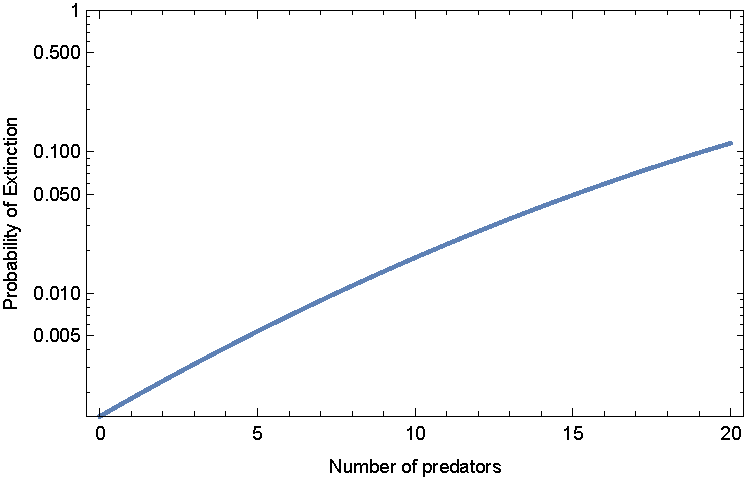
\includegraphics[width=0.45\textwidth]{extinction.pdf}
% \caption{
% The probability of extinction at time $t$ as a function of the number of predators consuming a given resource species $\omega_i(q)$. There is always \emph{some} risk of extinction even if a species has no predators, as $\omega_i(q=0) = 0.0014$.
% }
% \label{fig:ext}
% \end{figure} 



% Taken together, the community dynamics occur from a minimal set of rules:
% \begin{enumerate}
%   \item Colonization: At time-step $t$, determine whether eat/need threshold conditions are met for each species in the source pool that isn't currently in the community. Those passing the eat/need threshold conditions are \emph{potential colonizers}
%   \item Select at random a colonizing species and its attendant objects from the subset of potential colonizers
%   \item Extinction: Assess the probability of extinction for all species in the assembling community due to either resource overlap or predator load
%   \item Independently draw extinctions from a binomial distribution with a success probability equal to the extinction probabilities. Eliminate these species and any uniquely made objects from the community. These are \emph{primary extinctions}.
%   \item Re-assess whether eat/need threshold conditions are satisfied in the post-extinction community. Eliminate those species and any uniquely made objects from the community that do not meet threshold conditions. If further extinctions occur, continue to re-assess threshold conditions until all species meet the requirements. Combined, these are \emph{secondary extinctions}.
%   \item Time advances as t=t+1 and the process is repeated.
% \end{enumerate}
% 
% 




% 
% \textbf{Extinction via Resource Overlap} The matrix $\bm{A}$ is the asymmetrical adjacency matrix of eat and need interactions with rows corresponding to species and columns corresponding to both species \emph{and} objects.
% The number of users (eaters or needers) of each species/object is given by summing across columns resulting in the vector $\bm{x}$, and the number of species or objects eaten or consumed by each species is given by summing across rows resulting in the vector $\bm{y}$.
% 
% We calculate the number of species consuming or needing each of a species' possible resources (i.e. the number of species sharing a species' resources), not including itself by $\bm{z} = (\bm{A}\cdot\bm{x}) - \bm{y}$.
% Thus the average number of species sharing each species' resources is 
% $\bm{ro} = \bm{z}/\bm{y}$ (where division is element-by-element), and the average \emph{proportion} of species sharing each species' resources is given by ${\bm{RO}} = \bm{ro}/(S-1)$ where $S-1$ is the number of potential competitors in the community.
% 
% Thus, a species consuming/needing resources that have no other consumers/needers will have an ${\bm{RO}}=0$. In contrast, if all of a species' resources are shared by every other species in the community, ${\bm{RO}} = 1$.
% Partial overlap of resource use by other species ranges of course between 0 and 1.
% 
% The probability of extinction is assumed to be logistic as a function of ${\bm{RO}}$, where a value close to one will result in a probability of extinction close to one (and zero in the opposing case).
% Where the probability of extinction increases, and the slope of the increase are inputs of the model and largely set the steady state of the assembly process.
% 
% \textbf{Extinction via Predator Load} Assuming Lotka-Volterra predator-prey dynamics, a given resource $i$ has density $R_i$, growth rate $\alpha_i$, and carrying capacity $\kappa_i$.
% The consumption of this resource by $q$ non-specialist predators with equivalent steady state densities $P^*$ and attack rates $\beta$ results in the dimensionless steady state resource density $r_i^* = R_i^*/\kappa_i = 1 - q\epsilon_i$, where $\epsilon_i=\beta P^*/\alpha_i$ (see figure \ref{fig:lv} for an exemplary motif illustrating the described interactions).
% Thus, $\epsilon$ describes the relative impact of a single predator on the resource steady state, which decreases linearly with an increase in the number of predators $q$.
% Although our framework does not track changes in population densities, if we assume that the true resource density is normally distributed around $r^*$ with variance $\sigma^2$, the probability of extinction $\omega_i$ (defined as the probability that $r^* < 0$) has an exact solution of the form
% \begin{equation}
%   \omega_i(q) = \frac{1}{2}{\rm Erfc}\left(\frac{1-q\epsilon_i}{\sigma\sqrt{2}}\right).
% \end{equation}
% The probability of extinction for a resource increases sigmoidally with the number of predators on that resource, and the number of predators where the probability of extinction is $\omega=0.5$ is given by $q(\omega=0.5) = 1/\epsilon$.
% At each time-step, we calculate $\omega_i$ for each species in the assembled community and determine extinction by drawing from a binomial distribution where there is a single trial with success probability $\omega_i$.




% 
% 
% {\bf Community assembly without extinctions}
% In the context of community assembly, the niche space that is created by a given assemblage can be measured by evaluating the number of potential colonizers that can \emph{fit} within the assemblage from the species pool, fulfilling required assimilation and need threshold conditions.
% Because colonization without extinction does not account for resource limitation due to ever-expanding trophic loads of species that serve as resources for higher-trophic consumers, niche space is not reduced by packing more species into the community.
% However, because colonization from the mainland is a zero-sum event, with each successful colonization the number of potential future colonizers is reduced by one.
% Importantly, if a successful colonizer increases the number of potential future colonizers, this can be interpreted as functionally expanding the niche space of the community.
% 
% 
% 
% 
% Due to the competing effects of niche space expansion and species pool depletion, we find that the proportion of the species pool capable of successfully colonizing the assembling community is concave parabolic (Fig. \ref{fig_potcol}a).
% Early in the assembly process, the proportion of potential colonizers is equal to the proportion of species that are primary producers without an abundance of $n$ dependencies (too many need interactions precludes such primary producers from serving as initial colonizers).
% As assembly continues, niche space expands to a maximum, and then declines as the species pool diminishes and the community is filled.
% 
% 
% %Over pr(m)
% For a species pool of $400$, by changing the value of pr($m$) from 0.0001 to 0.002, we alter the proportion of engineers from ca. 0 to ca. 700.
% As the number of engineers is increased, the number of objects that they create -- and other species can interact with -- is likewise increased.
% For example, a single realization where $S=400$ species and pr(m)=$10^{-4}$ resulted in a $412\times412$ interaction matrix (400 species, 12 objects), while a realization with $S=400$ and pr(m)=$0.003$ resulted in a $1100\times1100$ interaction matrix (400 species, 700 objects).
% The former example generated a small number of engineers, each producing a single object, whereas the latter example generated a large number of engineers, each producing between 1-6 objects, with some objects being produced by multiple engineers.
% % 
% % \begin{figure*}[ht]
% % \centering
% % 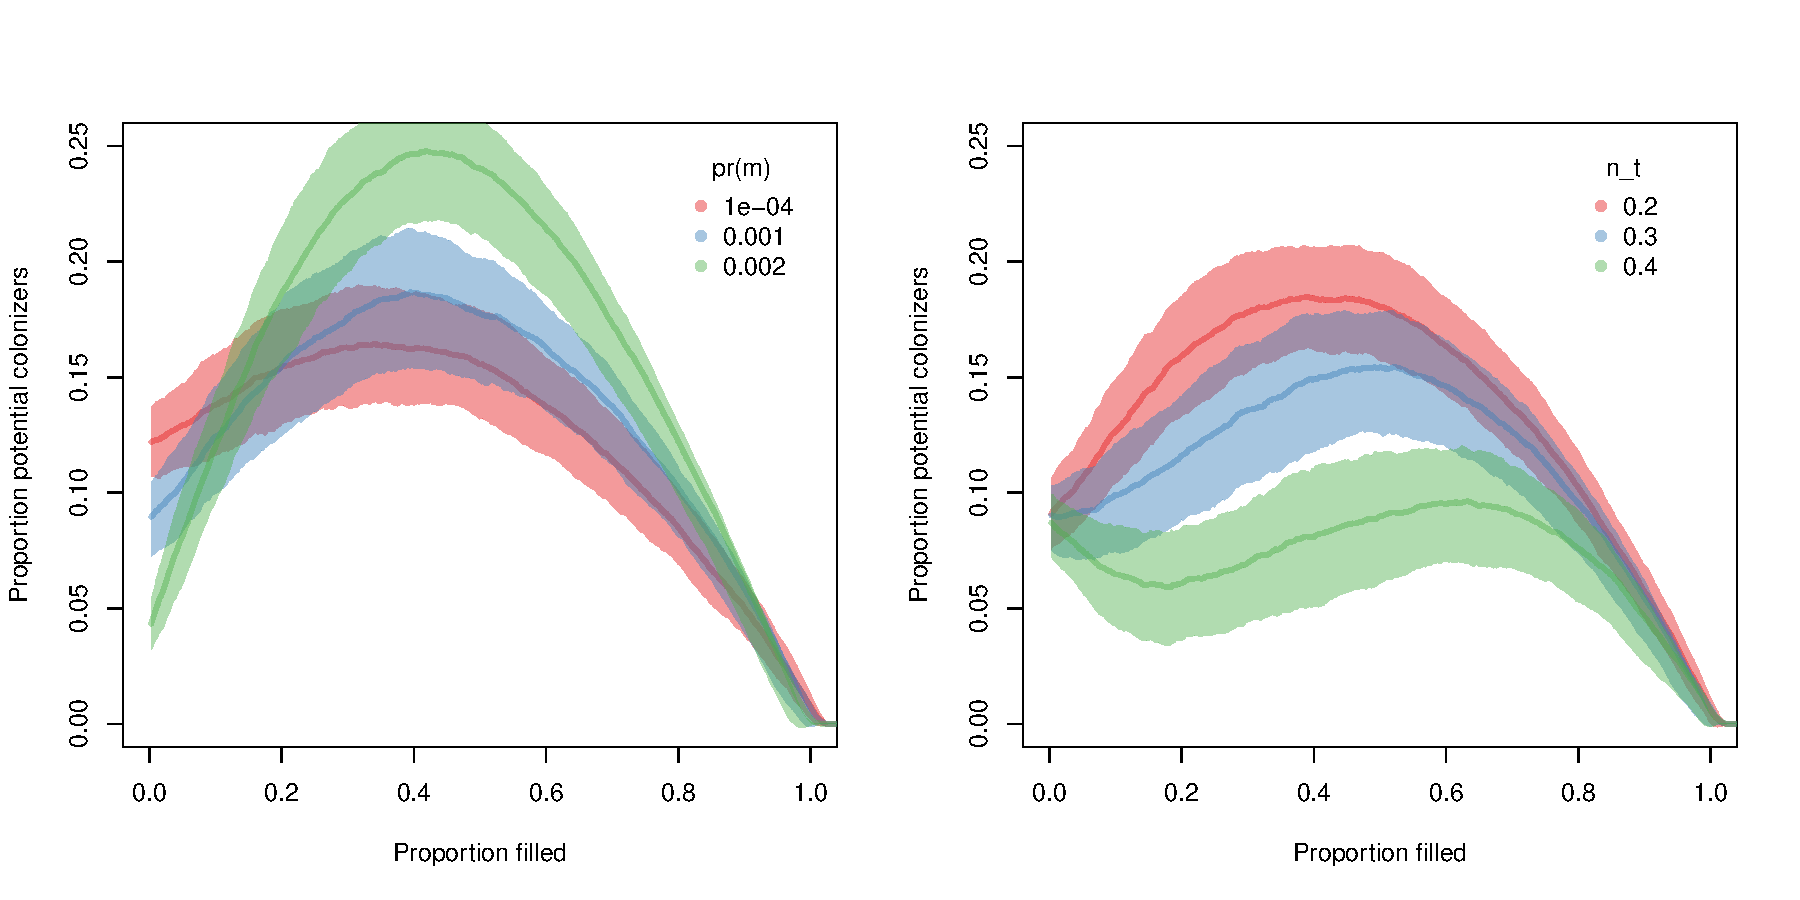
\includegraphics[width=0.9\textwidth]{fig_potcol_comb.pdf}
% % \caption{
% % a) Expansion of niche space (by counting the proportion of species that are capable of colonizing from the larger species pool) over systems with increasing number of engineers (increasing pr($m$)). b) Expansion of niche space over different need thresholds $n_t$. 
% % }
% % \label{fig_potcol}
% % \end{figure*} 
% 
% The effects of the proportion of engineers in the community on niche space expansion during assembly, and without the limiting forces of extinction, are substantial.
% While both limited-engineer and many-engineer systems resulted in a concave down niche expansion curve, the engineered system was different in three important ways.
% First, the many-engineer system began assembly with a smaller proportion of potential colonizers.
% This is due to the fact that there are many more interdependencies between species and objects, and as there are few objects carried over early in community development, the limitations on species are exaggerated.
% Second, the rate that niche space is expanded is higher for many-engineer communities
% Third, the production of objects by engineers nearly doubles the potential niche space (proportion of potential future colonizers) midway through assembly.
% Once there is a large enough base of colonizers in the assembling communities, there are enough objects present to facilitate rather than inhibit additional colonization opportunities.
% Thus, the influence of engineers during assembly - by creating more interdependencies between species and the objects they engineer - both constrains and promotes assembly at different stages of the process.
% 
% 
% %Over need_threshold
% Every species must satisfy at least one assimilate interaction, i.e. it must eat at least one other present species or basal resource.
% Moreover, every species must fulfill a certain proportion of its `need' interactions, set by the threshold parameter $n_t$.
% As $n_t$ increases, the interdependencies between species become more rigid during the assembly process, and this will serve to limit niche expansion.
% 
% However, the trajectory of niche expansion is more complex when $n_t$ is increased.
% Rather than simply lowering the proportion of potential colonizers, increasing $n_t$ results in a qualitatively different assembly process where niche space is first lowered, increased, and lowered again as the community is filled (Fig. \ref{fig_potcol}b).
% The initial niche space contraction results from a filling of the initial community with primary producers and their direct consumers.
% This lower trophic module fills without creating additional space for higher trophic level organisms due to the harsher restrictions given by a high $n_t$.
% Once a critical point in assembly is reached, the potential to add higher trophic level colonizers is attained, and niche space increases to a maximum, only to finally decrease as the species pool is used up.
% In some realizations, the community is never able to fill, resulting in a system without higher trophic levels.
% 
% Assembly where $n_t$ is large, and with moderate engineering, follows a 2-stage process.
% First, the system is colonized by primary producers.
% Once the lower trophic levels are filled and reach a critical point, niche expansion permits the colonization of higher trophic level colonizers.
% [Need to explore this more by calculating trophic level for each species - in progress]
% 
% 
% 
% 
% %Is there a diversity-stability link here?
% 
% 
% %Initial downward slope occurs because primary producers are used up. When it goes back up, there is enough of a base to build a larger community. Will have to check this will average trophic level over time (trophic module!!!)
% 
% 
% 
% 
% 
% {\bf Assembly with extinctions}
% % Negative effects of engineering at the scale of the community
% % The effect of engineers on extinction cascade size
% Examination of the assembly process that is regulated by extinctions due to changes in trophic load results in saturation of species richness over time (Fig. \ref{fig_traj}).
% Accordingly, the colonization and extinction dynamic result in regular fluctuations around a steady state community richness, where the size of the fluctuations (relative to the steady state value) strongly depends on $n_t$ and pr($(a,n$).
% 
% The average diversity of the system after an initial assembly process increases as the number of need interactions and/or need threshold $n_t$ are sufficiently low.
% This is intuitive because such a system has many more degrees of freedom and is free to expand to higher densities of species.
% Likewise, as pr($n$) and $n_t$ increase, species richness lowers nearly to zero, as does the average trophic level (check), resulting in a system dominated by primary producers and their immediate consumers.
% 
% 
% The system conforms to an expected Taylor's law relationship for lower species richness (<100), however follow different rules for higher richness (also corresponding to low pr($n$) and $n_t$.
% Here, species dependencies are low, such that primary extinctions due to predation will generally not result in a large number of secondary extinctions because the need threshold is not easily violated, and this reduces the magnitude of fluctuations.
% Accordingly, it is the same drivers that lead to high species richness (increased plasticity and/or fewer non-trophic dependencies) that also reduces the volatility of the system, thereby reducing variability.
% 
% 
% The magnitude of oscillations around the steady state richness is a measure of community instability and turnover.
% Although modification of pr($n$) and $n_t$ reveals a smooth and expected influence on the mean species richness of the community, the effect on the magnitude of fluctuations around the mean richness is more complex, and this is most evident in the coefficient of variation of community richness over time.
% The CV is maximized when $n_t$ is intermediate and the number of non-trophic dependencies is large.
% 
% % 
% % \begin{figure}
% % \centering
% % 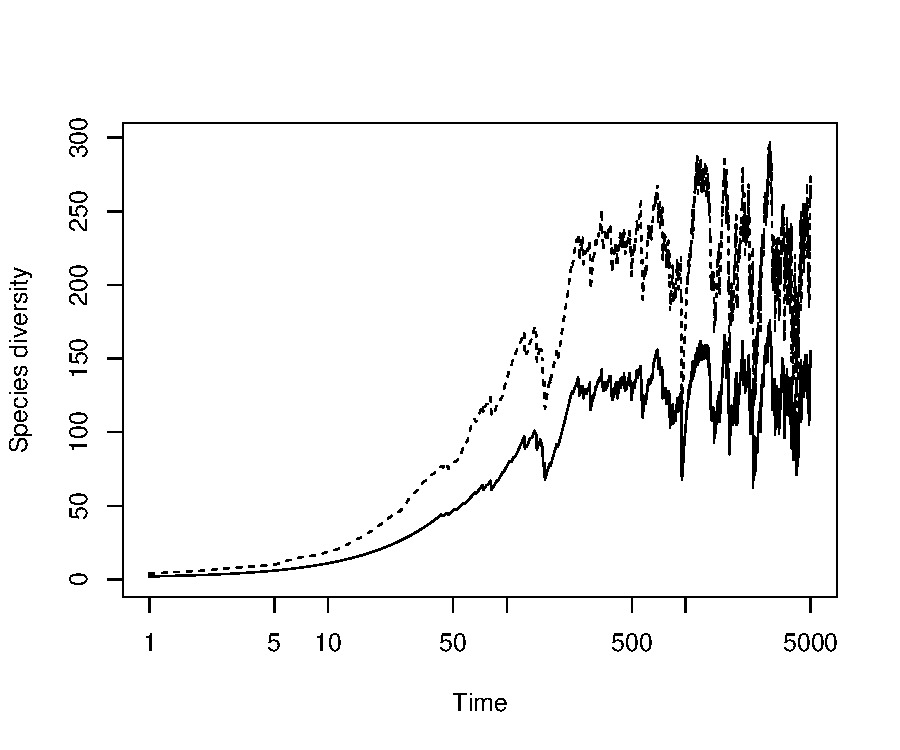
\includegraphics[width=0.45\textwidth]{fig_traj.pdf}
% % \caption{
% % The colonization and extinction dynamics of a community over time. The solid line denotes species richness; the dashed line denotes species+object richness.
% % }
% % \label{fig_traj}
% % \end{figure} 
% % 
% 
% 
% 
% {\bf Effects of engineers on community dynamics}
% We find that an increase in the number of engineers at time $t$ results in the potential for marginally larger extinction cascades at time $t+1$ (positive but weak correlations, Fig \ref{fig_corrobext}a).
% This weak positive correlation between the number of objects at time $t$ and extinction cascade size at time $t+1$ is due to the increasing interconnectedness that results from the higher number of objects relative to species in the system.
% Because the existence of a given object is tied to the species that makes them (one or multiple), the effects of primary extinctions are magnified.
% 
% % 
% % \begin{figure}
% % \centering
% % 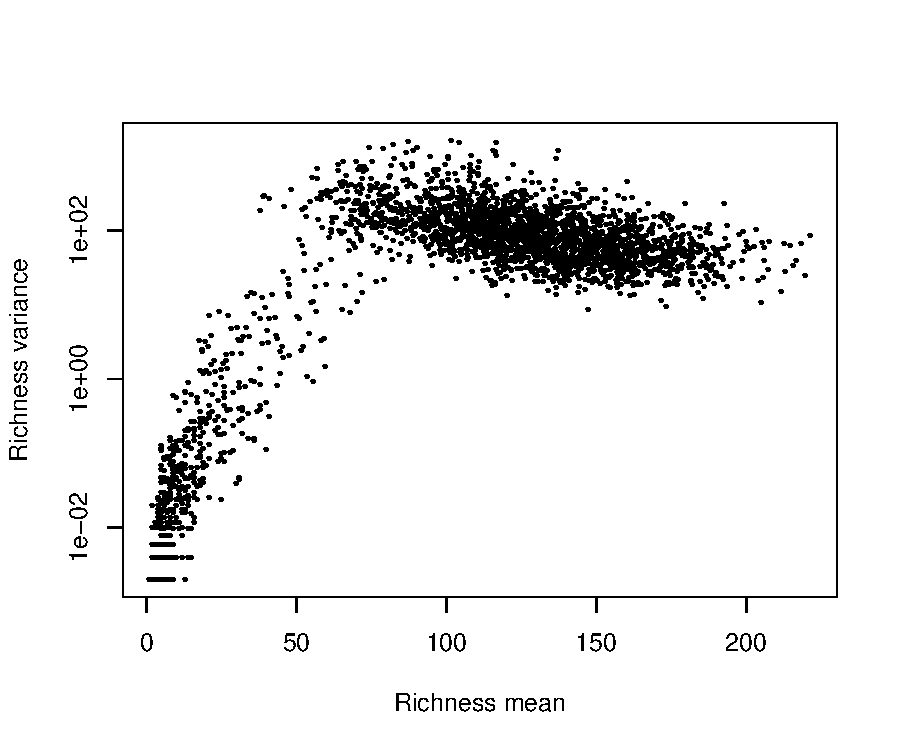
\includegraphics[width=0.45\textwidth]{fig_taylors.pdf}
% % \caption{
% % Relationship between mean species richness and the magnitude of fluctuations (SD) for communities with various values of pr($n$) and $n_t$.
% % }
% % \label{fig_traj}
% % \end{figure} 
% % 
% % 
% % \begin{figure}
% % \centering
% % 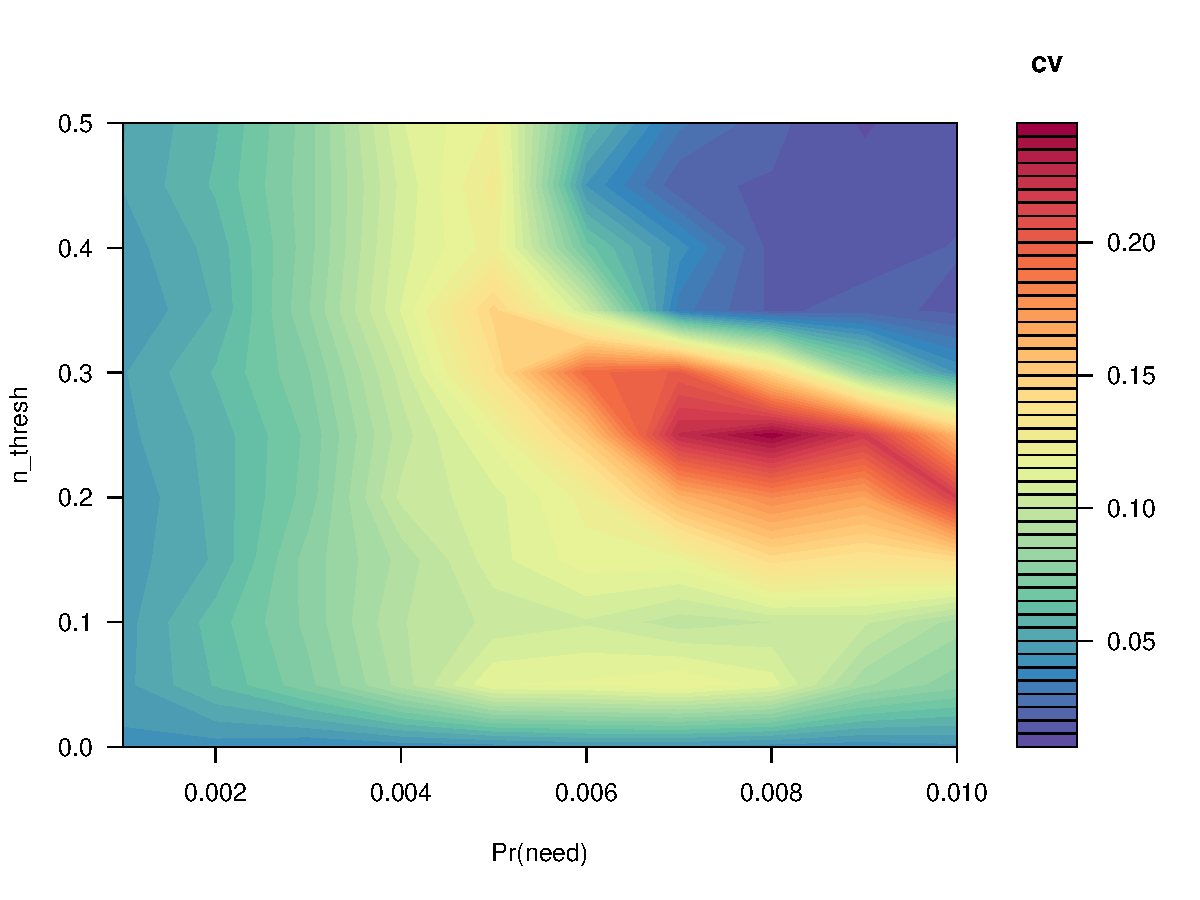
\includegraphics[width=0.45\textwidth]{fig_sen_nn.pdf}
% % \caption{Changes in community richness CV as a function of pr($n$) and $n_t$. 
% % }
% % \label{fig_sen_nn}
% % \end{figure} 
% % 
% 
% 
% 
% % The effect of engineering colonization facilitation
% The number of objects in the system at time $t$ (and by extension the number of engineers) is strongly positively correlated with the number of potential colonizers at time $t+1$.
% This correlation increases markedly with the proportion of engineers in the community.
% So from a species packing perspective, engineering enables successful colonization by increasing niche space, and this is particularly important for communities with a high proporiton of engineers.
% {\bf Colonization of engineers into a community both facilitates future colonization and increases the risks of larger extinction cascades}.
% This dual nature of ecosystem engineers may indicate short term/long term risks/gains?
% % 
% % 
% % \begin{figure*}[ht]
% % \centering
% % 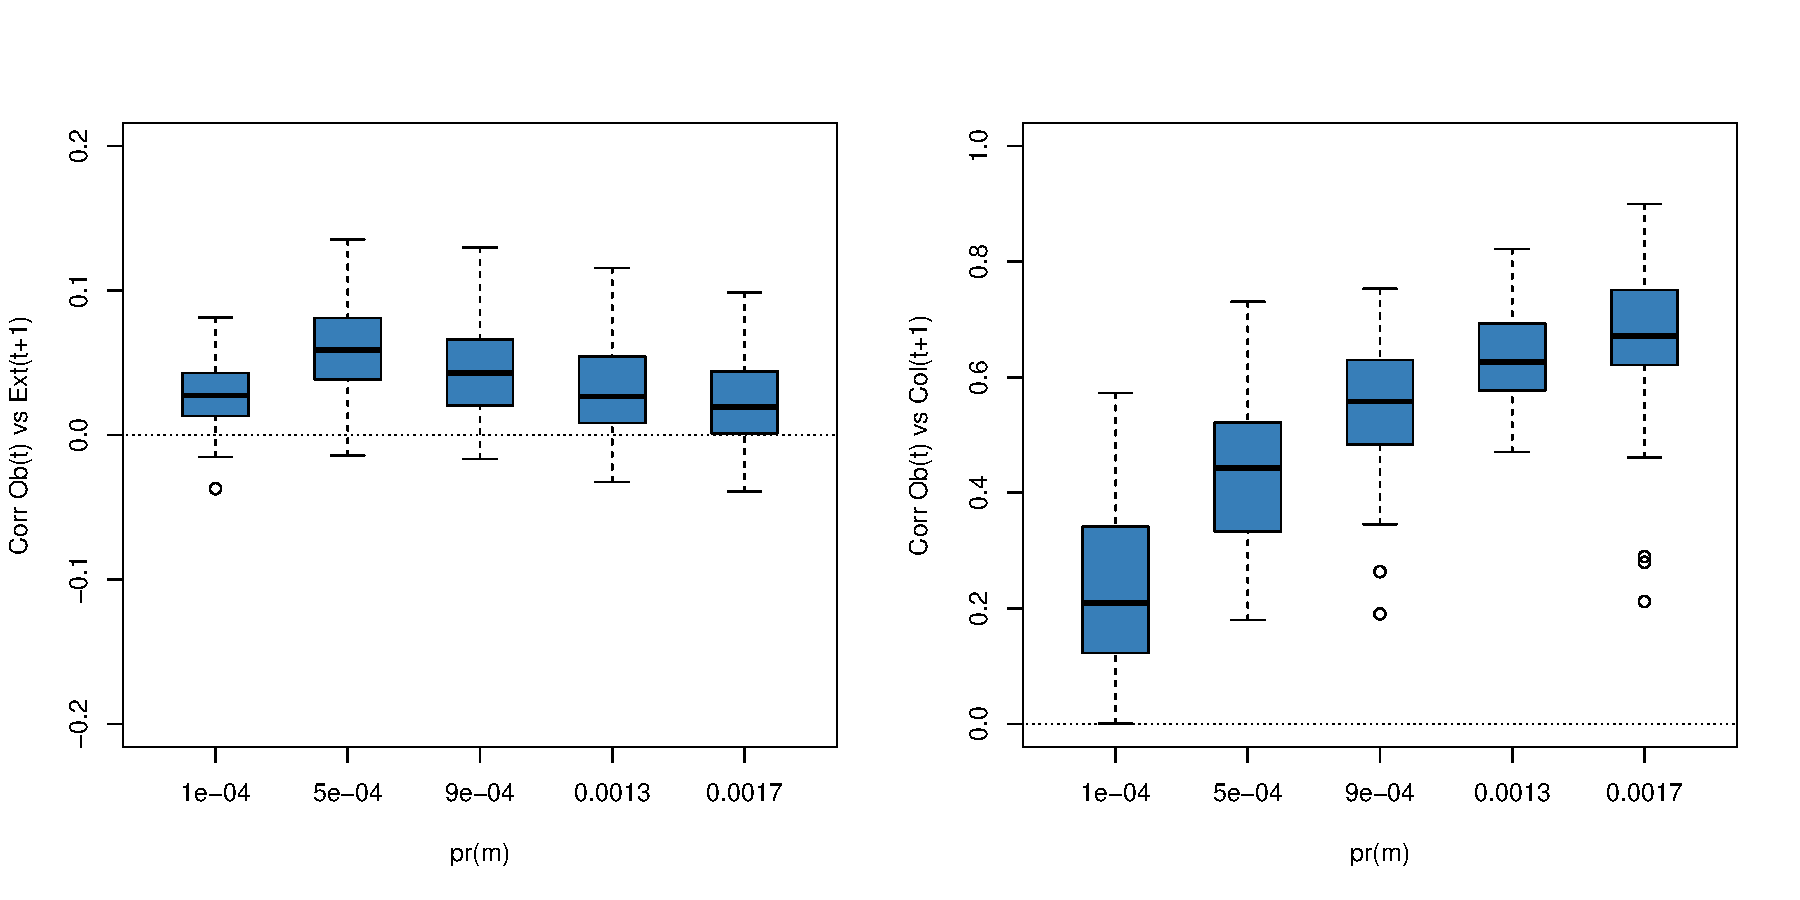
\includegraphics[width=0.75\textwidth]{fig_corrobext_tl2S.pdf}
% % \caption{
% % a) Correlations between objects at time $t$ and extinction cascade size at time $t+1$. b) Correlations between objects at time $t$ and the number of potential colonizers at time $t+1$.
% % }
% % \label{fig_corrobext}
% % \end{figure*} 
% 
% 
% Future things that I'm working on implementing (suggestions welcome!!!)
% \begin{enumerate}
% \item Calculate trophic level for each species
% \item Object decay - this is a big feature of engineered systems - that the objects they engineer can last longer than the species
% \item One potentially fruitful line of investigation would be to link this approach to random matrix theory - inclusion of objects should modify species effects on one another. I'm currently tracking both direct trophic and mutualistic adjacency matrices (where if species 1 makes object 1, and species 2 eats object 1, we can say species 2 indirectly eats species 1 - same for any other interaction type), but have not yet explored it - this would probably be good for a stand-alone paper - very little of engineering in food webs
% \item Priority effects - working on this - what species traits alter assembly dynamics?
% \end{enumerate}
% 


\end{document}
